\documentclass{article}

\usepackage[utf8]{inputenc}
\usepackage[dvipsnames]{xcolor}
\usepackage{lmodern}
\usepackage{graphicx}
\usepackage{longtable}
\usepackage{tabularx}
\graphicspath{ {../images/} }
\usepackage{imakeidx}
\makeindex[columns=3, title=Alphabetical Index, intoc]

\setlength{\arrayrulewidth}{.5mm}
\setlength{\tabcolsep}{5pt}
\renewcommand{\arraystretch}{2}

\usepackage{tabularx}
\usepackage{amsmath}
\usepackage{paralist}
\usepackage{enumitem}
\usepackage{hyperref} %\usepackage[hidelinks]{hyperref} %per togliere bordi rossi
\usepackage{makecell}
\usepackage{caption}
\usepackage[maxfloats=256]{morefloats}
\maxdeadcycles=1000

\usepackage[official]{eurosym}
\DeclareUnicodeCharacter{20AC}{\euro{}}

\author{Agosta, Belli, Emili, Giacchini, Luciani}

\begin{document}

\begin{center}
    \sffamily{\fontsize{50}{48} \selectfont \textcolor{red}{Nexi}\textcolor{green}{Fy}}
\end{center}

\begin{center}
    \itshape{\fontsize{20}{48} \selectfont streaming to your pocket}
\end{center}

\bigskip\bigskip\bigskip

\begin{flushleft}
    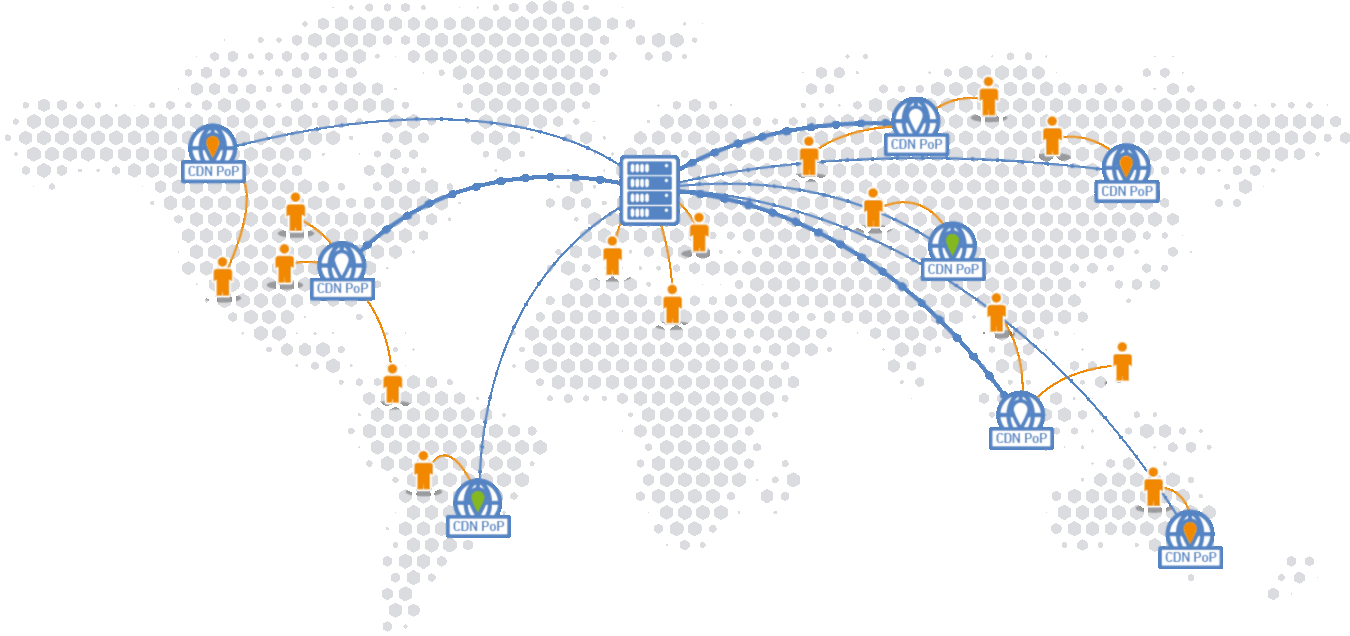
\includegraphics[scale=1]{../images/worldCDN.png}
\end{flushleft}

\bigskip\bigskip\bigskip

\begin{center}
    \itshape{\fontsize{30}{48} \selectfont Gestione dei Rischi}
\end{center}

\newpage
\printindex

\newpage
\section{\itshape{Gestione dei Rischi}}
Identificheremo qui i vari rischi per il progetto.\\
Ogni rischio ha una certa probabilità di verificarsi che varia tra: molto bassa, bassa, moderata, alta, molto alta; e provoca dei danni che possono essere: catastrofici, seri, tollerabili, insignificanti.\\
Useremo la tecnica RMMM (Risk Mitigation, Monitoring, Management) per la gestione dei rischi. Per ogni rischio individuato, verrà quindi trovata: 
\begin{itemize}
	\item una strategia di mitigation, per abbassare la probabilità che il rischio si verifichi, e ridurre anche i danni provacati dal rischio
	\item una strategia di monitoring per individuare cambiamenti nella probabilità del rischio
	\item una strategia di management per gestire il rischio, assumendo che questo si sia verificato
\end{itemize}
Inoltre classifichiamo i rischi in base agli aspetti che impattano: progetto, prodotto, business. \\
Identifichiamo i rischi con la convenzione RSC\_\textit{nome}. \\




%\begin{tabular}{|p{2.2cm}|p{9.6cm}| } 
% 	\hline
%	 \textbf{ID} & RSC\_ PerditaDati\\ [0.5ex] 
%	\hline
%	\textbf{Descrizione} & In seguito alla rottura di hard disk dei server, si perdono dati caricati dagli utenti o dati relativi agli utenti \\ 
%	\hline
%	\textbf{Probabilità} &  Molto bassa \\ 
%	\hline
%	\textbf{Impatto} &  Catastrofico \\ 
%	\hline
%	\textbf{Mitigation} & Distribuire i dati su più server ed effettuare backup (anche più di uno) di tutti i dati su server diversi. Sostituire hard disk difettosi. Progettare le varie funzionalità della piattaforma in modo che siano resistenti alle perdite di dati\\ 
%	\hline
%	\textbf{Monitoring} & Monitorare costantemente lo stato degli hard disk dei server, in modo da individuare eventuali problemi \\ 
%	\hline
%	\textbf{Management} & In caso di perdita di dati caricati dagli utenti, comunicarlo agli utenti in modo che possano eventualmente ricaricarli. In caso di dati persi quali informazioni sugli abbonamenti degli utenti, informare gli utenti e cercare di rimborsarli o offrire abbonamenti in omaggio (basandosi sui dati non persi) \\ 
%	\hline
%\end{tabular}

\begin{tabular}{|p{2.2cm}|p{9.6cm}| } 
 	\hline
	 \textbf{ID} & RSC\_ DifficoltàIntegrazioneServizi\\ [0.5ex] 
	\hline
	\textbf{Descrizione} & Diversi servizi esterni usati nella creazione della piattaforma (es: CDN, basi di dati, ecc), non si riescono a integrare come previsto\\ 
	\hline
	\textbf{Aspetto} &  Progetto, Prodotto\\ 
	\hline
	\textbf{Probabilità} &  Moderata\\ 
	\hline
	\textbf{Impatto} &  Serio\\ 
	\hline
	\textbf{Indicatori} & - Una funzionalità di un servizio esterno diventa deprecata\newline
				  - \'E necessario sfruttare più funzionalità del previsto da un servizio esterno \\
	\hline
	\textbf{Trigger} & Le funzionalità di un servizio esterno non possono essere usare insieme alle funzionalità di un altro servizio esterno\\
	\hline
	\textbf{Mitigation} & Prestare attenzione durante la fase di selezione dei servizi esterni, controllando che essi si integrino bene l'uno con l'altro\\ 
	\hline
	\textbf{Monitoring} & Controllare periodicamente eventuali aggiornamenti nei servizi effettuati dalle aziende esterne\\ 
	\hline
	\textbf{Management} & Contattare i fornitori per sapere se esistono soluzioni note per l'integrazione. In caso non esistessero soluzioni note per l'integrazione, si consideri di cambiare uno dei due servizi, in quanto implementare un'integrazione ad-hoc da zero in generale sarebbe più complicato e dispendioso\\ 
	\hline
\end{tabular}

\begin{tabular}{|p{2.2cm}|p{9.6cm}| }
 	\hline
	\textbf{ID} & RSC\_ CambiamentoRequisiti\\ [0.5ex] 
	\hline
	\textbf{Descrizione} & La specifica dei requisiti cambia durante il progetto \\ 
	\hline
	\textbf{Aspetto} &  Progetto\\
	\hline
	\textbf{Probabilità} &  Alta \\ 
	\hline
	\textbf{Impatto} &  Moderato \\ 
	\hline
	\textbf{Indicatori} & L'insieme di alcuni requisiti può portare a casi limite indesiderati\\
	\hline
	\textbf{Trigger} & Stakeholders non soddisfatti dei requisiti\\
	\hline
	\textbf{Mitigation} & Effettuare revisioni periodiche in modo da far emergere tempestivamente possibili cambiamenti nelle specifiche\\%Revisionare attentamente l'analisi dei requisiti all'inizio del progetto, in modo da abbassare la probabilità di grandi cambiamenti.\\ 
	\hline
	\textbf{Monitoring} & Durante le revisioni e l'analisi dei requisiti, immaginare situazioni limite che potrebbero verificarsi\\%Effettuare revisioni periodiche in modo da far emergere tempestivamente possibili cambiamenti nelle specifiche\\ 
	\hline
	\textbf{Management} & Se le modifiche ai requisiti non comportano un grande ritardo nel progetto, o si tratta di requisiti di alta priorità, allora adattare il progetto ai nuovi requisiti. Se dopo aver aggiunto i nuovi requisiti la durata del progetto supera di molto quella precedentemente prevista, eliminare requisiti secondari per restare nei tempi \\ 
	\hline
\end{tabular}


\clearpage
\begin{tabular}{|p{2.2cm}|p{9.6cm}| }
 	\hline
	\textbf{ID} & RSC\_ IndisponibilitàPersonale\\ [0.5ex] 
	\hline
	\textbf{Descrizione} & Alcuni elementi del personale potrebbero essere indisponibili in alcuni periodi del progetto\\ 
	\hline
	\textbf{Aspetto} &  Progetto \\
	\hline
	\textbf{Probabilità} &  Alta \\ 
	\hline
	\textbf{Impatto} &  Tollerabile \\ 
	\hline
	\textbf{Indicatori} & Malcontento del personale\\
	\hline
	\textbf{Trigger} & -\\
	\hline
	\textbf{Mitigation} & Fare una previsione di eventuali giorni di assenza mentre si pianifica lo sviluppo oltre che incoraggiare i dipendenti a comunicare in anticipo eventuali indisponibilità già previste (tipicamente indisponibilità non dovute a malattie) \\ 
	\hline
	\textbf{Monitoring} & Mantenere una comunicazione tra dipendenti e resto dell'azienda, per venire a conoscenza il prima possibile di indisponibilità e monitorare periodicamente quanto prodotto effettivamente dai membri rispetto quello che avrebbero dovuto produrre secondo il piano in modo da rilevare ritardi\\ 
	\hline
	\textbf{Management} & Se l'indisponibilità è per un breve periodo, distribuire il lavoro del personale assente sugli altri dipendenti. Se l'indisponibilità si protrae troppo a lungo, assumere nuovi dipendenti per un certo periodo o addirittura valutare una riprogrammazione delle scadenza\\ 
	\hline
\end{tabular}


\begin{tabular}{|p{2.2cm}|p{9.6cm}| }
 	\hline
	\textbf{ID} & RSC\_ CasiD'UsoErrati\\ [0.5ex] 
	\hline
	\textbf{Descrizione} & I requisiti non vengono compresi nella realizzazione dei casi d'uso.\\ 
	\hline
	\textbf{Aspetto} &  Progetto\\
	\hline
	\textbf{Probabilità} &  Bassa \\ 
	\hline
	\textbf{Impatto} &  Serio \\ 
	\hline
	\textbf{Indicatori} & Cambiamento nei requisiti\\
	\hline
	\textbf{Trigger} & Incomprensione nell'interpretazione dei requisiti\\
	\hline
	\textbf{Mitigation} & Revisionare attentamente l'analisi dei requisiti prima di definire i casi d'uso.\\ 
	\hline
	\textbf{Monitoring} & Effettuare revisioni periodiche in modo da far emergere tempestivamente possibili fraintendimenti delle specifiche\\ 
	\hline
	\textbf{Management} & Ridefinire i casi d'uso in modo da renderli coerenti con i requisiti corretti. Se dopo aver modificato i casi d'uso la durata del progetto supera di molto quella precedentemente prevista, eliminare requisiti secondari per restare nei tempi \\ 
	\hline
\end{tabular}
\clearpage
\begin{tabular}{|p{2.2cm}|p{9.6cm}| }
	\hline
   \textbf{ID} & RSC\_ TecnologiaObsoleta\\ [0.5ex] 
   \hline
   \textbf{Descrizione} & Durante l'implementazione del progetto, le tecnologie che si intendono utilizzare diventano obsolete \\ 
   \hline
   \textbf{Aspetto} &  Progetto \\
   \hline
   \textbf{Probabilità} & Moderata\\ 
   \hline
   \textbf{Impatto} & Tollerabile\\
	\hline
	\textbf{Indicatori} & - Piattaforme con le stesse difficoltà di Nexify si preparano ad un cambio di tecnologia\\
	\hline
	\textbf{Trigger} & - Una tecnologia diversa da quella adottata si consolida come la più adatta\\
   \hline
   \textbf{Mitigation} & Scegliere, al momento dello sviluppo iniziale, tecnologie aggiornate e che abbiano dimostrato di essere affidabili in altri progetti \\ 
   \hline
   \textbf{Monitoring} & Tenere traccia periodicamente delle tecnologie esistenti, e di possibili nuovi aggiornamenti o cambiamenti che avvengono \\ 
   \hline
   \textbf{Management} & Effettuare un’analisi per capire se la tecnologia originale è ancora adatta allo svolgimento del compito per cui è stata scelta. In caso negativo, deve essere sostituita con una tecnologia più adatta.\\ 
   \hline
\end{tabular}


\begin{tabular}{|p{2.2cm}|p{9.6cm}| }
	\hline
   \textbf{ID} & RSC\_ DimensioneSoftwareSottostimata\\ [0.5ex] 
   \hline
   \textbf{Descrizione} & La dimensione del software da produrre viene sottostimata \\ 
   \hline
   \textbf{Aspetto} &  Progetto \\
   \hline
   \textbf{Probabilità} & Moderata\\ 
   \hline
   \textbf{Impatto} & Serio\\
	\hline
	\textbf{Indicatori} & - Le stime iniziali sulla dimensione del software si rivelano non attendibili \\
	\hline
	\textbf{Trigger} & - Le stime correnti portano a superare la scadenza dell'iterazione corrente\\
   \hline
   \textbf{Mitigation} & Svolgere in maniera accurata le fase di analisi e pianificazione del progetto, in modo da stimare una dimensione il più vicino possibile a quella reale. Inoltre per ogni iterazione aggiungere dei giorni aggiuntivi per fare fronte a eventuali ritardi dovuti a stime sbagliate \\ 
   \hline
   \textbf{Monitoring} & Durante lo sviluppo, controllare periodicamente che la dimensione del software rimanga contenuta, in base a quanto è stato pianificato nelle fasi iniziali\\ 
   \hline
   \textbf{Management} & Qualora, durante lo sviluppo, il software dovesse superare la dimensione prestabilita per quello stadio, si deve effettuare una nuova stima che tenga conto delle nuove informazioni acquisite. Successivamente si deve rivedere la pianificazione del progetto, eventualmente apportando modifiche laddove la dimensione del software risulta maggiore di quella stimata inizialmente \\ 
   \hline
\end{tabular}

\begin{tabular}{|p{2.2cm}|p{9.6cm}| } 
 	\hline
	 \textbf{ID} & RSC\_ SovraccaricoCDN\\ [0.5ex] 
	\hline
	\textbf{Descrizione} & Le richieste effettuate dagli utenti superano il carico massimo sopportabile dalla CDN \\ 
	\hline
   	\textbf{Aspetto} &  Prodotto \\
	\hline
	\textbf{Probabilità} &  Moderata \\ 
	\hline
	\textbf{Impatto} &  Tollerabile \\ 
	\hline
	\textbf{Indicatori} & - Il numero di richieste di contenuti contemporanee aumenta \newline
						  - Guasti della CDN\\
	\hline
	\textbf{Trigger} & - Il numero di richieste ad un nodo è maggiore delle richieste gestibili\newline
					   - Non ci sono abbastanza nodi per gestire la richieste in una certa area\\
	\hline
	\textbf{Mitigation} & Viene sottoscritta una SLA che impone delle penali e permette di rescindere il contratto nel caso in cui la qualit\'a del servizio non venga rispettata. Inoltre si definiscono nella SLA i tempi di risoluzione del disservizio ed estensione delle capacit\'a della CDN. \\ 
	\hline
	\textbf{Monitoring} & Osservare periodicamente il numero di richieste ricevute, e i file di log dei nodi della CDN, in modo da individuare possibili sovraccarichi. Inoltre si valutano eventuali segnalazioni degli utenti riguardanti la qualit\'a del servizio\\ 
	\hline
	\textbf{Management} & Nel caso in cui la qualit\'a del servizio della CDN non rispettasse la qualit\'a definita nel contratto si richieder\'a un'incremento delle prestazioni. Se il fornitore del servizio non riuscisse a risolvere il problema si può rescindere il contratto e riscuorete le penali. \\ 
	\hline
\end{tabular}


\begin{tabular}{|p{2.2cm}|p{9.6cm}| } 
 	\hline
	 \textbf{ID} & RSC\_ DegradoQualitàContenuti\\ [0.5ex] 
	\hline
	\textbf{Descrizione} & Contenuti amatoriali di scarsa qualità abbondano sulla piattaforma, portando a un degrado della qualità dei contenuti offerti. \\ 
	\hline
   	\textbf{Aspetto} &  Prodotto \\
	\hline
	\textbf{Probabilità} &  Bassa \\ 
	\hline
	\textbf{Impatto} &  Tollerabile \\ 
	\hline
	\textbf{Indicatori} & - L'abbasssamento della quota di sottoscrizione di abbonamenti abilitati alla pubblicazione \newline
						  - Diminuzione della popolarit\'a della piattaforma\\
	\hline
	\textbf{Trigger} & - La quota di iscrizione ad abbonamenti partner permette l'iscrizione a pubblicatori non affidabili\newline
					   - La piattaforma non è popolare e ai pubblicatori di alto calibro non conviene pubblicare contenuti (affidabili) sulla piattaforma\\
	\hline
	\textbf{Mitigation} & Scegliere attentamente i costi che gli utenti devono pagare per poter pubblicare contenuti. \newline
						  Investire nella pubblicit\'a della piattaforma \\ 
	\hline
	\textbf{Monitoring} & Controlli periodici sui contenuti presenti sulla piattaforma. \newline
						  Controllare il calibro dei pubblicatori iscritti alla piattaforma \\ 
	\hline
	\textbf{Management} & Aumentare il prezzo richiesto per abilitare la pubblicazione di prodotti \newline
						  Fare pubblicit\'a per nuovi abbonamenti\\ 
	\hline
\end{tabular}


\begin{tabular}{|p{2.2cm}|p{9.6cm}| }
 	\hline
	\textbf{ID} & RSC\_ DurataSottostimata\\ [0.5ex] 
	\hline
	\textbf{Descrizione} & La durata dell'iterazione corrente viene sottostimata \\ 
	\hline
	\textbf{Aspetto} &  Progetto \\
	\hline
	\textbf{Probabilità} & Basso\\ 
	\hline
	\textbf{Impatto} & Serio\\
	\hline
	\textbf{Indicatori} & - Problemi emersi durante svoglimento del lavoro prefissato\\
	\hline
	\textbf{Trigger} & - La gestione dei problemi sorti provoca uno slittamento dei tempi che non permette di ultimare il lavoro prefissato nell'iterazione corrente\\
	\hline
	\textbf{Mitigation} & Lasciare qualche giorno in più del previsto in ogni iterazione, in modo da far fronte a eventuali errori di stima per una certa iterazione\\ 
	\hline
	\textbf{Monitoring} & Esaminare periodicamente l'andamento dell'iterazione corrente, in modo da individuare potenziali situazioni che portano a superare la durata stimata dell'iterazione\\ 
	\hline
	\textbf{Management} & Se è la prima iterazione che è stata sottostimata, si può distribuire il lavoro in eccesso sull'iterazione successiva, in quanto è improbabile aver sottostimato due iterazioni consecutive. Se è la seconda iterazione di fila che è stata sottostimata, considerare la rimozione di requisiti meno importanti, in quanto si accumulerebbe troppo lavoro continuando a rimandare sulle fasi successive \\ 
	\hline
\end{tabular}


\begin{tabular}{|p{2.2cm}|p{9.6cm}| }
 	\hline
	\textbf{ID} & RSC\_ RiduzioneBudget\\ [0.5ex] 
	\hline
	\textbf{Descrizione} & Il budget disponibile viene ridotto durante il progetto\\ 
	\hline
	\textbf{Aspetto} &  Business\\
	\hline
	\textbf{Probabilità} & Molto basso\\ 
	\hline
	\textbf{Impatto} & Catastrofico\\
	\hline
	\textbf{Indicatori} & - Introduzione di costi non previsti \newline
						  - Riduzione dei finanziamenti\\
	\hline
	\textbf{Trigger} & - Nuovi costi emergono rispetto a quelli precedentemente stabiliti eccedendo una certa soglia\newline
					   - L'ammontare dei finanziamenti ricevuti diminuisce rispetto al minimo previsto inizialmente\\
	\hline
	\textbf{Mitigation} & Richiedere inizialmente un budget leggermente più alto del necessario, in modo da coprire eventuali, piccole, riduzioni\\
	\hline
	\textbf{Monitoring} & Controllare periodicamente che l'avanzamento del progetto segua i costi previsti, e sfruttare eventuali condizioni che portano a risparmio\\ 
	\hline
	\textbf{Management} & Ridimensionare il progetto in base al nuovo budget, rimuovendo le funzionalità meno importanti\\ 
	\hline
\end{tabular}

\renewcommand\theadfont{}

\newpage
\noindent{\large \textbf{Revisioni 7}} \\ \\
\begin{tabular}{|c | c | c | c|} 
 	\hline
	 Numero & Data & Descrizione \\ [0.5ex] 
	\hline\hline
	1 & 07/02/2020 & Stesura iniziale \\ 
	\hline
	2 & 16/02/2020 & Modificato monitoring e management di REQ\_M\_DurataSottostimata \\
	\hline
	3 & 15/03/2020 & Aggiunti trigger e indicatori di rischio \\
	\hline
\end{tabular}
\index{Index}

\end{document}
